\chapter{Chart types}
Charts can be created by calling the appropriate chart plug-in constructor with: the identifier for the canvas element to use, the data, and an options object. The following example shows how to create a simple bar chart, add a title and subtitle, and set its size.
\begin{verbatim}
  var c = chart.bar('canvas', data, {
    title: 'Q1 Sales',
    subtitle: 'By Region'
  });

  c.bounds({
    width: 200,
    height: 100
  });

  c.draw();
\end{verbatim}

Because each chart plug-in is a "subclass" of the chart component, the \code{preferredSize}, \code{minimumSize}, \code{bounds}, and other methods are available and can be used to---for example---set a chart to its preferred size (taking the aspect ratio into account.) The \code{bar} plugin name in the above example can be replaced by any of the following chart plug-ins that come with the library:

\begin{description}
\item[bar] The bar chart plug-in supports categories and subcategories, in both horizontal and vertical orientations. It can also display stacked bar charts.
\item[scatter] The scatter chart plug-in supports single or multiple categories with two variables.
\item[line] The line chart plug-in supports categories and subcategories.
\item[histogram] The histogram supports multiple categories but not subcategories.
\item[plot] The plot chart plug-in supports plotting a single function with one or two variables.
\end{description}

Using these chart plug-ins it is possible to display all the relationships defined in Chapter 2.7. The following list describes how each relationship maps to a plug-in appropriate for displaying that relationship.

\begin{description}
\item[Nominal comparison] Nominal comparisons should almost always be encoded as a bar chart.
\item[Time series] When there are few time subdivisions and many categories, a line chart with a line for each category is a good solution. When there are few time subdivisions and few categories a bar chart should be used. Finally,  time series with many time subdivisions should be encoded as a line chart.
\item[Ranking] A ranking relationship should be encoded as an ordered nominal comparison, and as such displayed in a bar or column chart.
\item[Part to whole] Part to whole relationships are best displayed as stacked bar charts.
\item[Deviation] When there are few categories a deviation relationship can be displayed as bars, but when there are many categories a line chart should be used.
\item[Distribution] When a distribution has a single variable and few values a histogram is recommended. When the distribution has more than one variable, it is best to use a scatter chart. If the distribution has a single variable and many values it should be displayed as a line chart. 
\item[Correlation] Correlation relationships are best displayed as scatter charts.
\item[Function] Functions should be plotted using the plot chart, or if a function is very simple, a line chart.
\end{description}

Of course these solutions are only suggestions, as long as a chart plug-in accepts the input it will try to draw the data. If that is not sufficient it is always possible to extend either the available data relationships or add new chart plug-ins through the plug-in extension mechanism.

The following sections detail the visual output of each chart type and its input values.

\section{Bar Chart}
The most simple bar chart is shown in Figure \ref{barsimple}, which displays the (fictitious) employee turnover in various departments. Its input data object is as follows:
\begin{verbatim}
  var d = {
    categories: ['Sales', 'Engineering', 'Marketing', 'HR'],
    data: [1.5, 3, 2.2, -0.3]
  };
\end{verbatim}
Note that the negative value results in a chart with a zero baseline and correctly drawn negative bar. The axis range and tick marks are automatically generated by the axis algorithm described earlier.
\begin{figure}[H]
	\centering
	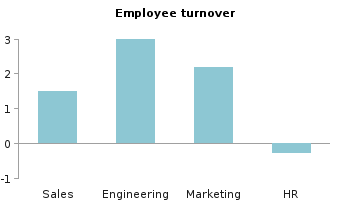
\includegraphics[width=.6\linewidth]{barsimple}
	\caption{Bar chart without sub categories}
	\label{barsimple}
\end{figure}

The width of the bars is defined by the available space, which means that creating a smaller chart creates thinner bars. The ratio between the bar width and spacing between the bars is always kept at $1:1$, which is the recommended ratio \cite{few04}.

The chart in Figure \ref{rankingbar} shows a horizontal bar chart, with the categories on the vertical axis and values on the horizontal axis. In this case the chart is used to display a ranking relationship with the largest value at the top of the chart. The data input is shown below.

\begin{verbatim}
  var d = {
    categories: ['West', 'South', 'East', 'North'],
    data: [38, 25, 22, 15]
  };
\end{verbatim}

The default bar orientation is vertical. To draw bars in a horizontal orientation, the \code{reverse: true} boolean should be added to the options object passed to the bar chart constructor.

\begin{figure}[H]
	\centering
	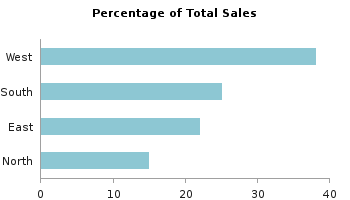
\includegraphics[width=.6\linewidth]{barrank}
	\caption{A ranking bar chart}
	\label{rankingbar}
\end{figure}

The next bar chart variation is one with subcategories, shown in Figure \ref{subcategory}. This chart has two main categories, "Treasury Bonds" and "AAA Municipal Bonds", and also two subcategories "Ten-Year Yields" and "Two-Year Yields". Subcategory bars are drawn together, while the main categories are separated by the width of one bar.

\begin{figure}[H]
	\centering
	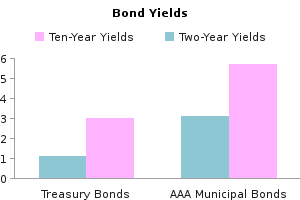
\includegraphics[width=.5\linewidth]{subcategory}
	\caption{A bar chart with subcategories and legend}
	\label{subcategory}
\end{figure}

Because the legend only has two items it is drawn above the chart, right below the title. If the legend had too many items it would have been drawn on the right side of the chart. The data object for this chart looks as follows:

\begin{verbatim}
  var d = {
    categories: ['Treasury Bonds', 'AAA Municipal Bonds'],
    subcategories: ['Two-Year Yields', 'Ten-Year Yields'],
    data: [
      [1.11, 3],
      [3.1, 5.7],
    ]
  };
\end{verbatim}

The last bar chart variant, a stacked bar chart, is shown in Figure \ref{stackedbar}. This chart can display a part to whole relationship, and in this case, a percentage of total sales. The input to a stacked bar chart is identical to a bar chart with multiple categories.

\begin{verbatim}
  var d = {
    categories: ['Q1', 'Q2'],
    subcategories: ['West', 'East', 'South', 'North'],
    data: [
      [38, 22, 15, 25],
      [25, 27, 20, 28]
    ]
  };
\end{verbatim}

The user can add the \code{stacked: true} boolean to the options object to draw any bar chart with subcategories as a stacked bar chart. The plug-in automatically adds up the values to create the maximum value of the "whole" and creates an appropriate axis. A legend is added as usual.

\begin{figure}[H]
	\centering
	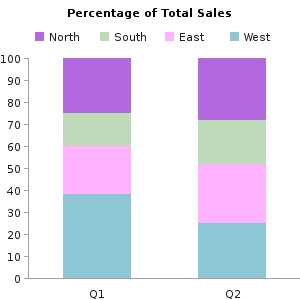
\includegraphics[width=.5\linewidth]{stacked}
	\caption{A bar stacked bar chart}
	\label{stackedbar}
\end{figure}


\section{Scatter Chart}

The scatter chart plug-in displays the correlation between values. Figure \ref{scatter} displays Anscombe's quartet of datasets \cite{anscombe73, tufte01}. Each set has an identical mean, variance, correlation and linear regression. These datasets were used by Anscombe to argue the usefulness of plotting data in charts.

\begin{figure}[H]
	\centering
	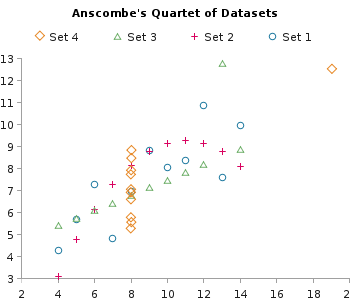
\includegraphics[width=.6\linewidth]{scatter}
	\caption{Scatter chart with multiple categories}
	\label{scatter}
\end{figure}

The chart plugin uses different symbols for each dataset and also draws each symbol in a different colour to help distinguish them from each other. Again a legend is used to label the different sets. The data object is not reproduced here because it is rather large.

\section{Line Chart}
Line charts can be used to plot time series and simple functions. Figure \ref{simpleline} is an example of a simple time series with a single category: "Sales per year". The data object for this chart is very basic, two arrays, one for the categories and one for the values belonging to each category.
\begin{verbatim}
  var d = {
    categories: ['2001', '2002', '2003', '2004', '2005', '2006', '2007', '2008'],
    data: [13000, 13400, 14000, 16000, 14100, 12700, 15000, 16000]
  };
\end{verbatim}

Note that the line does not start at the zero point and the end point of each line segment is located directly above the category label, indicating the line symbolizes discrete values instead of continuous values.

\begin{figure}[H]
\centering
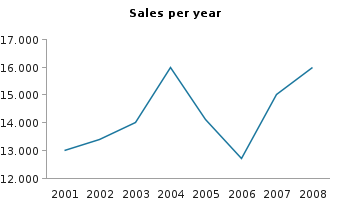
\includegraphics[width=.6\linewidth]{linesimple}
\caption{Line chart with single category}
\label{simpleline}
\end{figure}

Figure \ref{multiline} shows a line chart used to draw a time series with multiple categories. The lines for the different categories leave enough space for drawing the legend directly onto the chart, a practice recommended over a normal legend \cite{few04}. If the lines ended at the same points or very close to each other the line chart plug-in would have opted to use a legend instead. The data object is shown below:

\begin{verbatim}
  var d = {
    categories: ['2001', '2002', '2003', '2004', '2005', '2006'],
    subcategories: ['Engineering', 'Marketing', 'HR', 'R&D'],
    data: [
        [1200, 2000, 4000, 4500, 5000, 6300],
        [2000, 4000, 3200, 6000, 7000, 7500],
        [1000, 1500, 1000, 1000, 1800, 1800],
        [1800, 2000, 2100, 2300, 2000, 2700]
    ]
  };
\end{verbatim}

\begin{figure}[H]
\centering
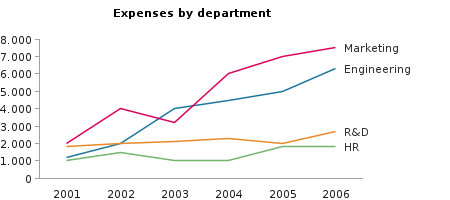
\includegraphics[width=.8\linewidth]{linemultiple}
\caption{Line chart with multiple categories}
\label{multiline}
\end{figure}


\section{Histogram}

The histogram chart plug-in supports plotting simple histograms. It accepts categories but not subcategories. Figure \ref{histogram} shows a histogram that plots the frequency versus the height (in feet) of black cherry trees. Because the histogram chart type does not support subcategories a simple grey colour is chosen as the fill colour.

\begin{figure}[H]
\centering
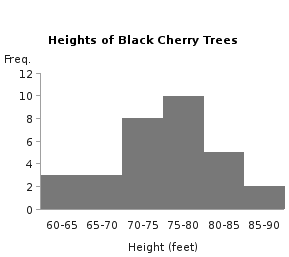
\includegraphics[width=.5\linewidth]{histogram}
\caption{Histogram with individual axis labels}
\label{histogram}
\end{figure}

Note that this chart also uses axis labels for both the horizontal and vertical axis, a feature that is supported on all chart types (because it is part of the canvas component, and not specific to the histogram plug-in.)

\section{Function plotting}
The plot chart plug-in supports plotting of mathematical equations in a certain range. Figure \ref{plots} shows: a) a simple plot of $y(t) = sin(t)$ and b) a plot of the "Rhodonea curve" defined by $r = cos(4\theta)$, plotted in polar coordinates. The sine plot also shows non-numeric and Unicode support in labels.

\begin{figure}[H]
	\centering
	\subfloat[Sine wave]{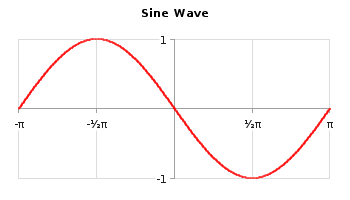
\includegraphics[width=0.5\textwidth]{sin}}
	\subfloat[Rhodonea curve]{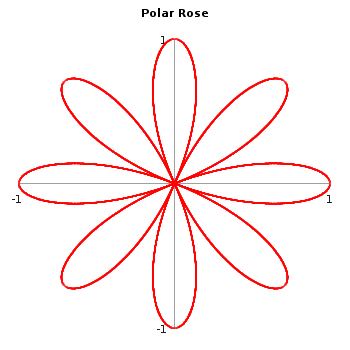
\includegraphics[width=0.5\textwidth]{rose}}
	\caption{Function plots in Cartesian and polar coordinates}
	\label{plots}
\end{figure}

These figures are plotted using interval arithmetic. The basic idea behind plotting using interval arithmetic is to subdivide the range in which to plot a function into four sections. Each section is evaluated in turn for a possible solution using the user supplied function. If a solution is found, the subdivisions with a solution are again subdivided into four sections and the algorithm repeats. If no solution is found in a particular section it does not need further examination \cite{shou05, fateman92, martin02}.

The effect of these recursive subdivisions is that the algorithm basically operates as a quad-tree algorithm \cite{finkel74}. It keeps subdividing until it either reaches a user-specified depth level or the subdivisions are smaller than one screen pixel. At that point it will plot a pixel on that location. This pixel is then guaranteed to contain the correct solution. This also means that plots are always correct, in that they have no missing singularities or artifacts that are difficult to plot using other methods.

\begin{figure}[H]
\centering
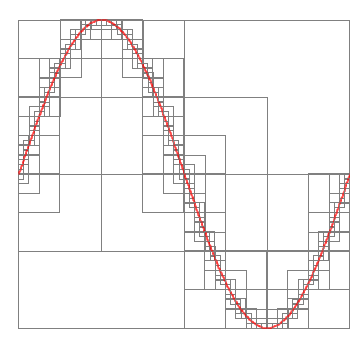
\includegraphics[width=.5\linewidth]{interval}
\caption{Quadtree generated by the interval arithmetic algorithm}
\label{quadtree}
\end{figure}

Figure \ref{quadtree} shows the algorithm at work for a simple sine wave. The big empty rectangles do not have a solution in them, the smaller rectangles are further subdivided until the subdivision becomes smaller than a screen pixel, at which point the pixel is coloured red. The number of subdivisions in this image is limited to a size of four pixels so as to clearly demonstrate the algorithm.

